\documentclass{beamer}
% PREAMBLE TAKEN FROM OTHER PRESENTATION, PERHAPS OBSOLETE
%\usetheme{Rochester}
\usepackage{graphicx}
\setbeamerfont{footnote}{size=\tiny}
\beamertemplatenavigationsymbolsempty
% END DUBIOUS PREAMBLE

\setbeamertemplate{caption}[numbered]
\usepackage{tikz}

\title[Artificial Intelligence and Games]{Artificial Intelligence and Games}
\author{Will Bolton}
\date{\today}

\begin{document}
\titlepage % SLIDE 0

\begin{frame} % SLIDE 1
\frametitle{History}
\begin{figure}
	\centering
	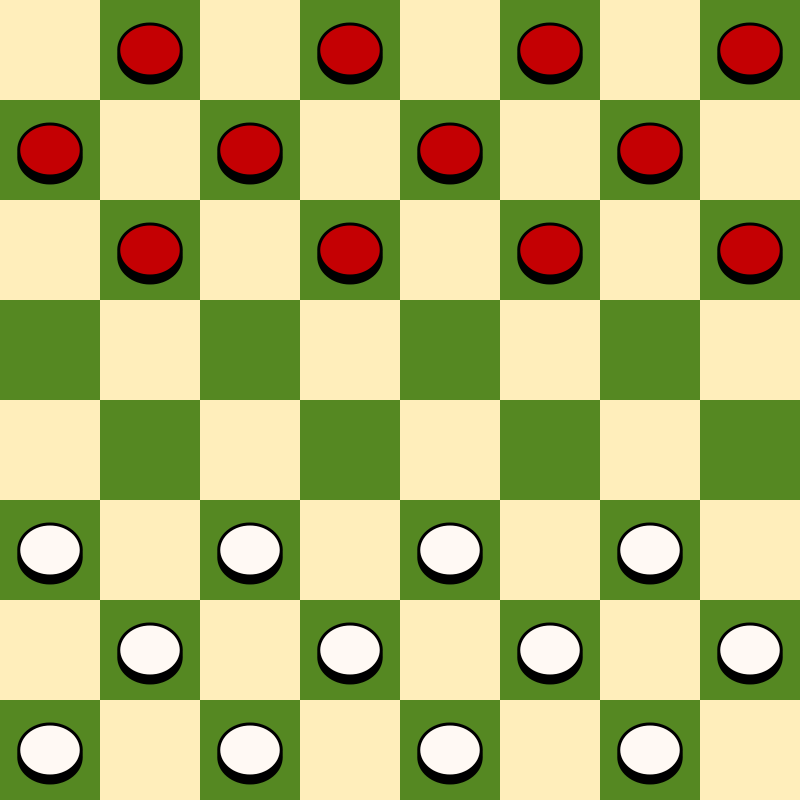
\includegraphics[width=0.5\textwidth]{images/draughts.png}
	\caption{Starting position for English Draughts}
	\label{draughts}
\end{figure}
\end{frame}

\begin{frame} % SLIDE 2
\frametitle{The Turk}
\begin{figure}
	\centering
	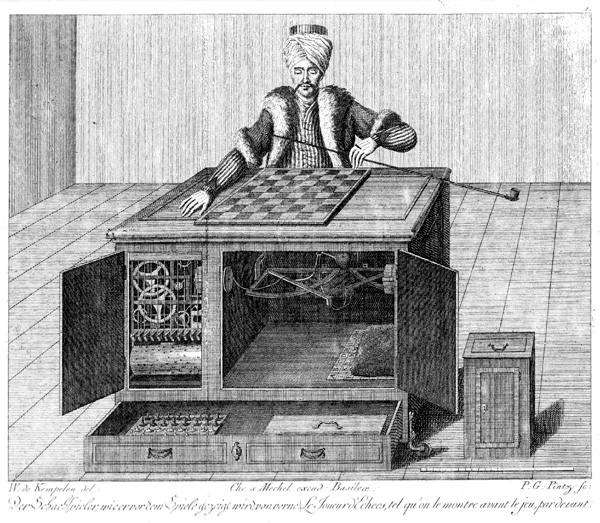
\includegraphics[width=0.5\textwidth]{images/turk.jpg}
	\caption{Engraving of the Mechanical Turk}
	\label{turk}
\end{figure}
\end{frame}

\begin{frame} % SLIDE 3
\frametitle{Noughts and Crosses}
\begin{figure}
	\centering
	\begin{tikzpicture}
		\draw (0,1) -- (3,1);
		\draw (0,2) -- (3,2);
		\draw (1,0) -- (1,3);
		\draw (2,0) -- (2,3);
	\end{tikzpicture}
\end{figure}
\end{frame}

\begin{frame} % SLIDE 4
\frametitle{Early Chess Computers}
\begin{figure}
	\centering
	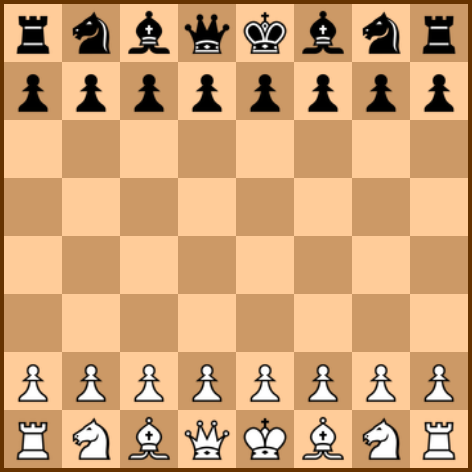
\includegraphics[width=0.5\textwidth]{images/chessinitial.png}
	\caption{Starting position for chess \cite{chessgames}}
	\label{chessinitial}
\end{figure}
\end{frame}

\begin{frame} % SLIDE 5
\frametitle{Deep Blue}
\begin{figure}
	\centering
	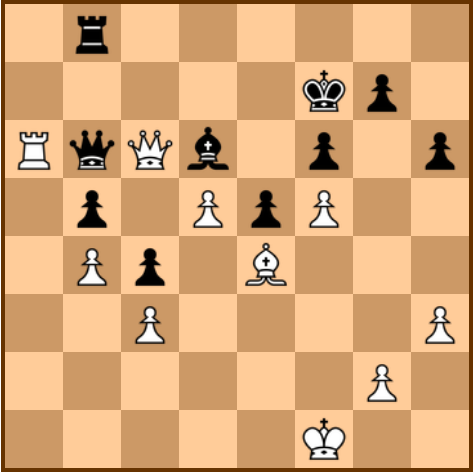
\includegraphics[width=0.5\textwidth]{images/deep-blue.png}
	\caption{Final position of the 1997 rematch \cite{chessgames}}
	\label{deep-blue}
\end{figure}
\end{frame}

\begin{frame} % SLIDE 6a
\frametitle{Go}
\begin{figure}
	\centering
	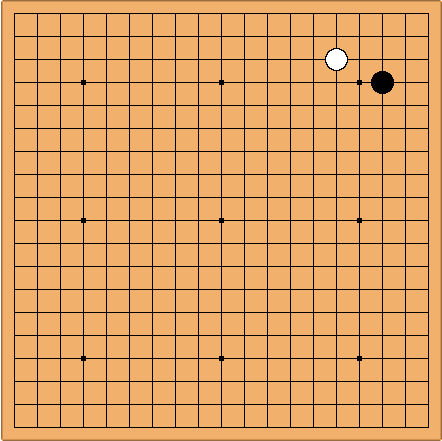
\includegraphics[width=0.5\textwidth]{images/go.png}
	\caption{The $19\times19$ board on which Go is played}
	\label{go}
\end{figure}
\end{frame}

\begin{frame} % SLIDE 6b
\frametitle{Go}
45,193,640,626,062,205,213,735,739,171,550,309,047,984,050,718 \cite{chesspositions}
\end{frame}

\begin{frame} % SLIDE 6c
\frametitle{Go}
208,168,199,381,979,984,699,478,633,344,862,770,286,522,453,884,\\
530,548,425,639,456,820,927,419,612,738,015,378,525,648,451,698,\\
519,643,907,259,916,015,628,128,546,089,888,314,427,129,715,319,\\
317,557,736,620,397,247,064,840,935 \cite{gopositions}
\end{frame}

\begin{frame} % SLIDE 7
\frametitle{Alpha Go}
\begin{figure}
	\centering
	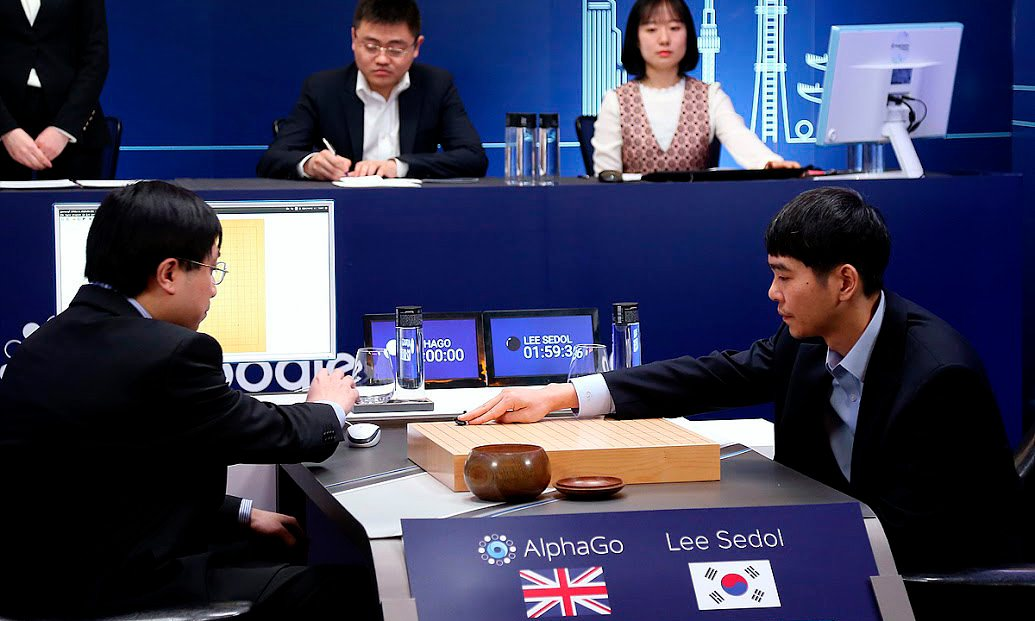
\includegraphics[width=0.7\textwidth]{images/alphagomatch.jpg}
	\caption{Lee Sedol playing AlphaGo}
	\label{alphagomatch}
\end{figure}
\end{frame}

\begin{frame} % SLIDE 8
\frametitle{Bibliography}
\begin{thebibliography}{9}
	\bibitem{chessgames}
	Chess diagrams - http://www.chessgames.com/

	\bibitem{chesspositions}
	Chess positions - http://tromp.github.io/chess/chess.html

	\bibitem{gopositions}
	Go positions - http://tromp.github.io/go/legal.html

	\bibitem{alphago}
	Mastering the game of Go with deep neural networks and tree search\\
	Silver, David et al.\\
	Nature, 2016
\end{thebibliography}
\end{frame}

\end{document}
